% Options for packages loaded elsewhere
\PassOptionsToPackage{unicode}{hyperref}
\PassOptionsToPackage{hyphens}{url}
%
\documentclass[
]{article}
\usepackage{amsmath,amssymb}
\usepackage{lmodern}
\usepackage{iftex}
\ifPDFTeX
  \usepackage[T1]{fontenc}
  \usepackage[utf8]{inputenc}
  \usepackage{textcomp} % provide euro and other symbols
\else % if luatex or xetex
  \usepackage{unicode-math}
  \defaultfontfeatures{Scale=MatchLowercase}
  \defaultfontfeatures[\rmfamily]{Ligatures=TeX,Scale=1}
\fi
% Use upquote if available, for straight quotes in verbatim environments
\IfFileExists{upquote.sty}{\usepackage{upquote}}{}
\IfFileExists{microtype.sty}{% use microtype if available
  \usepackage[]{microtype}
  \UseMicrotypeSet[protrusion]{basicmath} % disable protrusion for tt fonts
}{}
\makeatletter
\@ifundefined{KOMAClassName}{% if non-KOMA class
  \IfFileExists{parskip.sty}{%
    \usepackage{parskip}
  }{% else
    \setlength{\parindent}{0pt}
    \setlength{\parskip}{6pt plus 2pt minus 1pt}}
}{% if KOMA class
  \KOMAoptions{parskip=half}}
\makeatother
\usepackage{xcolor}
\usepackage[margin=1in]{geometry}
\usepackage{color}
\usepackage{fancyvrb}
\newcommand{\VerbBar}{|}
\newcommand{\VERB}{\Verb[commandchars=\\\{\}]}
\DefineVerbatimEnvironment{Highlighting}{Verbatim}{commandchars=\\\{\}}
% Add ',fontsize=\small' for more characters per line
\usepackage{framed}
\definecolor{shadecolor}{RGB}{248,248,248}
\newenvironment{Shaded}{\begin{snugshade}}{\end{snugshade}}
\newcommand{\AlertTok}[1]{\textcolor[rgb]{0.94,0.16,0.16}{#1}}
\newcommand{\AnnotationTok}[1]{\textcolor[rgb]{0.56,0.35,0.01}{\textbf{\textit{#1}}}}
\newcommand{\AttributeTok}[1]{\textcolor[rgb]{0.77,0.63,0.00}{#1}}
\newcommand{\BaseNTok}[1]{\textcolor[rgb]{0.00,0.00,0.81}{#1}}
\newcommand{\BuiltInTok}[1]{#1}
\newcommand{\CharTok}[1]{\textcolor[rgb]{0.31,0.60,0.02}{#1}}
\newcommand{\CommentTok}[1]{\textcolor[rgb]{0.56,0.35,0.01}{\textit{#1}}}
\newcommand{\CommentVarTok}[1]{\textcolor[rgb]{0.56,0.35,0.01}{\textbf{\textit{#1}}}}
\newcommand{\ConstantTok}[1]{\textcolor[rgb]{0.00,0.00,0.00}{#1}}
\newcommand{\ControlFlowTok}[1]{\textcolor[rgb]{0.13,0.29,0.53}{\textbf{#1}}}
\newcommand{\DataTypeTok}[1]{\textcolor[rgb]{0.13,0.29,0.53}{#1}}
\newcommand{\DecValTok}[1]{\textcolor[rgb]{0.00,0.00,0.81}{#1}}
\newcommand{\DocumentationTok}[1]{\textcolor[rgb]{0.56,0.35,0.01}{\textbf{\textit{#1}}}}
\newcommand{\ErrorTok}[1]{\textcolor[rgb]{0.64,0.00,0.00}{\textbf{#1}}}
\newcommand{\ExtensionTok}[1]{#1}
\newcommand{\FloatTok}[1]{\textcolor[rgb]{0.00,0.00,0.81}{#1}}
\newcommand{\FunctionTok}[1]{\textcolor[rgb]{0.00,0.00,0.00}{#1}}
\newcommand{\ImportTok}[1]{#1}
\newcommand{\InformationTok}[1]{\textcolor[rgb]{0.56,0.35,0.01}{\textbf{\textit{#1}}}}
\newcommand{\KeywordTok}[1]{\textcolor[rgb]{0.13,0.29,0.53}{\textbf{#1}}}
\newcommand{\NormalTok}[1]{#1}
\newcommand{\OperatorTok}[1]{\textcolor[rgb]{0.81,0.36,0.00}{\textbf{#1}}}
\newcommand{\OtherTok}[1]{\textcolor[rgb]{0.56,0.35,0.01}{#1}}
\newcommand{\PreprocessorTok}[1]{\textcolor[rgb]{0.56,0.35,0.01}{\textit{#1}}}
\newcommand{\RegionMarkerTok}[1]{#1}
\newcommand{\SpecialCharTok}[1]{\textcolor[rgb]{0.00,0.00,0.00}{#1}}
\newcommand{\SpecialStringTok}[1]{\textcolor[rgb]{0.31,0.60,0.02}{#1}}
\newcommand{\StringTok}[1]{\textcolor[rgb]{0.31,0.60,0.02}{#1}}
\newcommand{\VariableTok}[1]{\textcolor[rgb]{0.00,0.00,0.00}{#1}}
\newcommand{\VerbatimStringTok}[1]{\textcolor[rgb]{0.31,0.60,0.02}{#1}}
\newcommand{\WarningTok}[1]{\textcolor[rgb]{0.56,0.35,0.01}{\textbf{\textit{#1}}}}
\usepackage{graphicx}
\makeatletter
\def\maxwidth{\ifdim\Gin@nat@width>\linewidth\linewidth\else\Gin@nat@width\fi}
\def\maxheight{\ifdim\Gin@nat@height>\textheight\textheight\else\Gin@nat@height\fi}
\makeatother
% Scale images if necessary, so that they will not overflow the page
% margins by default, and it is still possible to overwrite the defaults
% using explicit options in \includegraphics[width, height, ...]{}
\setkeys{Gin}{width=\maxwidth,height=\maxheight,keepaspectratio}
% Set default figure placement to htbp
\makeatletter
\def\fps@figure{htbp}
\makeatother
\setlength{\emergencystretch}{3em} % prevent overfull lines
\providecommand{\tightlist}{%
  \setlength{\itemsep}{0pt}\setlength{\parskip}{0pt}}
\setcounter{secnumdepth}{-\maxdimen} % remove section numbering
\ifLuaTeX
  \usepackage{selnolig}  % disable illegal ligatures
\fi
\IfFileExists{bookmark.sty}{\usepackage{bookmark}}{\usepackage{hyperref}}
\IfFileExists{xurl.sty}{\usepackage{xurl}}{} % add URL line breaks if available
\urlstyle{same} % disable monospaced font for URLs
\hypersetup{
  pdftitle={Analyzing the Structure of a Neural Network},
  pdfauthor={Samuel Richards},
  hidelinks,
  pdfcreator={LaTeX via pandoc}}

\title{Analyzing the Structure of a Neural Network}
\usepackage{etoolbox}
\makeatletter
\providecommand{\subtitle}[1]{% add subtitle to \maketitle
  \apptocmd{\@title}{\par {\large #1 \par}}{}{}
}
\makeatother
\subtitle{An Applied Approach with Theoretical Backing}
\author{Samuel Richards}
\date{}

\begin{document}
\maketitle

\hypertarget{foundations}{%
\subsection{Foundations}\label{foundations}}

Start with the overall structure of a very simple neural network.\\
- Include an illustration.\\
How pixel values are assessed in the case of image classification.\\
Similar assessment for other types of data.

Then, dive into the individual neuron description.

The Multi-Layer Perceptron

\begin{itemize}
\tightlist
\item
  Actually composed of sigmoid neurons
\item
  Input (data), hidden layer(s), output

  \begin{itemize}
  \tightlist
  \item
    Hidden layers do:
  \end{itemize}
\item
  Image data: each pixel is an input value

  \begin{itemize}
  \tightlist
  \item
    Can get extremely large
  \end{itemize}
\item
  Other data: each observation is an input value -also can get extremely
  large
\item
  One hidden layer is sufficient to make accurate predictions from
  training data. More hidden layers increase the depth of the network,
  and often calls for fewer units per layer. Deeper networks are better
  at generalizing test data, but are harder to optimize
  \cite{Goodfellow-et-al-2016} \emph{(Re-address this claim down the
  road)}
\end{itemize}

The Perceptron

\begin{itemize}
\tightlist
\item
  artificial neuron developed by Frank Rosenblatt in the 1950s
  \cite{nielsen}
\item
  Takes several binary inputs and outputs a single binary output:
\item
  Output is determined by the weighted sum of all input values with
  respective weights
\end{itemize}

\[
Y = 
\begin{cases}
0 \text{ if } \sum_i^n w_ix_i \le D \\
1 \text{ if } \sum_i^n w_ix_i > D
\end{cases}
\] Where \(i\) can be any number \(n\) of input values composed in the
network and \(D\) is the threshold value that the weighted sum is
matched with to determine the binary output \(Y\).

Because these inputs are calculated by computers, and computers like
vectors, the notation is adjusted to allow for proper computation.. In
addition, Rosenblatt introduced a bias (check source) to shift the
function to a clean threshold of \(D = 0\). \[
Y = 
\begin{cases}
0 \text{ if } w_i \cdot x_i + b_i \le 0 \\
1 \text{ if } w_i \cdot x_i + b_i > 0
\end{cases}
\]

This is represented by the \emph{step function}.

\begin{Shaded}
\begin{Highlighting}[]
\NormalTok{step }\OtherTok{\textless{}{-}} \ControlFlowTok{function}\NormalTok{(x)\{}
  \FunctionTok{ifelse}\NormalTok{ (x }\SpecialCharTok{\textless{}=} \DecValTok{0}\NormalTok{,}\DecValTok{0}\NormalTok{,}\DecValTok{1}\NormalTok{) }
\NormalTok{\}}

\NormalTok{f }\OtherTok{\textless{}{-}} \FunctionTok{seq}\NormalTok{(}\SpecialCharTok{{-}}\DecValTok{8}\NormalTok{,}\DecValTok{8}\NormalTok{, }\AttributeTok{length=}\DecValTok{1000}\NormalTok{)}

\FunctionTok{plot}\NormalTok{(f,}\FunctionTok{step}\NormalTok{(f), }\AttributeTok{type =} \StringTok{\textquotesingle{}s\textquotesingle{}}\NormalTok{, }\AttributeTok{lwd =} \DecValTok{8}\NormalTok{, }\AttributeTok{main=}\StringTok{"Step Function"}\NormalTok{, }\AttributeTok{xlab =} \StringTok{" "}\NormalTok{, }\AttributeTok{ylab =} \StringTok{" "}\NormalTok{, }\AttributeTok{ylim =} \FunctionTok{c}\NormalTok{(}\DecValTok{0}\NormalTok{,}\DecValTok{1}\NormalTok{), }\AttributeTok{col =} \StringTok{"turquoise"}\NormalTok{, }\AttributeTok{frame.plot =}\NormalTok{ T)}
\end{Highlighting}
\end{Shaded}

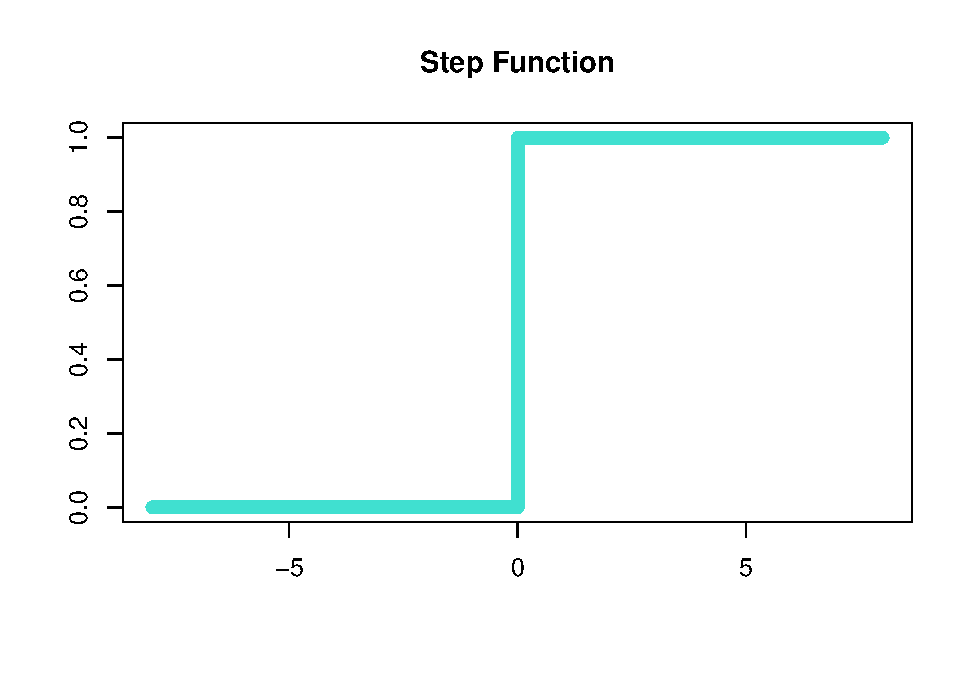
\includegraphics{ANN_files/unnamed-chunk-1-1.pdf}

The problem with the perceptron is that a small change in weight can
cause the outcome to change dramatically, since the output is binary.

Sigmoid neuron

\begin{itemize}
\tightlist
\item
  modified from perceptrons so that small changes in weights or bias
  causes a small change in output
\item
  not a binary output, rather an output of the interval {[}0,1{]}
\item
  Sigmoid function
\end{itemize}

\[
\sigma(z) = \frac{1}{1+e^{-z}} \\
\] Where \(z\) is the same equation from the perceptron
\(w \cdot x + b\). That is, \[
\sigma(w_i \cdot x_i + b_i) = \frac{1}{1+e^{-\sum_i^n w_i \cdot x_i - b}}
\] For each \(i\) weight \(w_i\), bias \(b_i\), and input \(x_i\).

Which is represented by the \emph{Sigmoid Function}
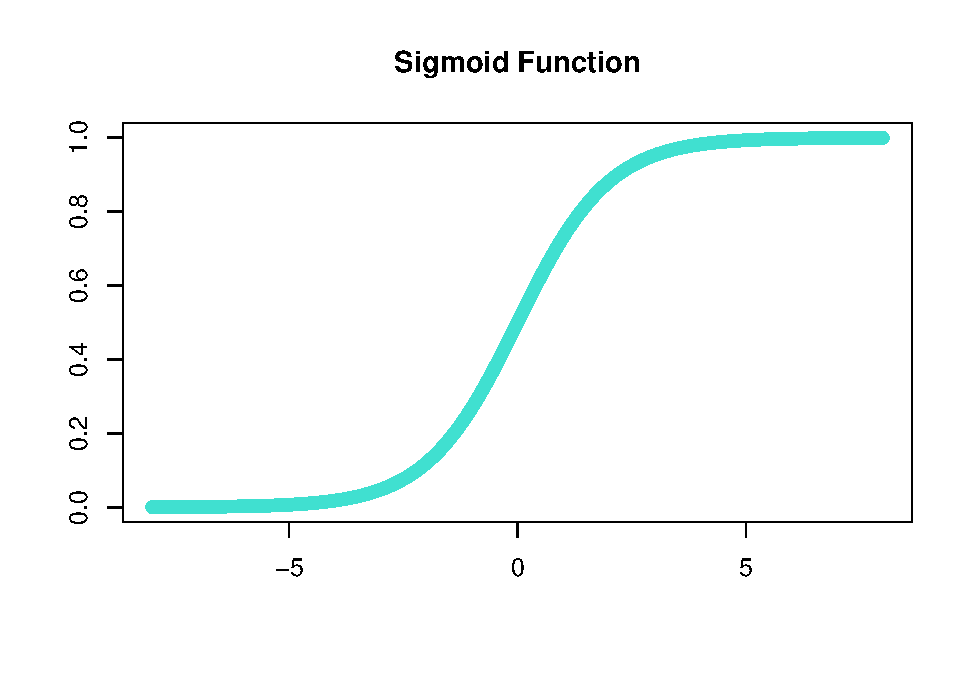
\includegraphics{ANN_files/unnamed-chunk-2-1.pdf}

\hypertarget{activation-functions}{%
\subsection{Activation Functions}\label{activation-functions}}

(Write about other activation functions and discuss their differences.)

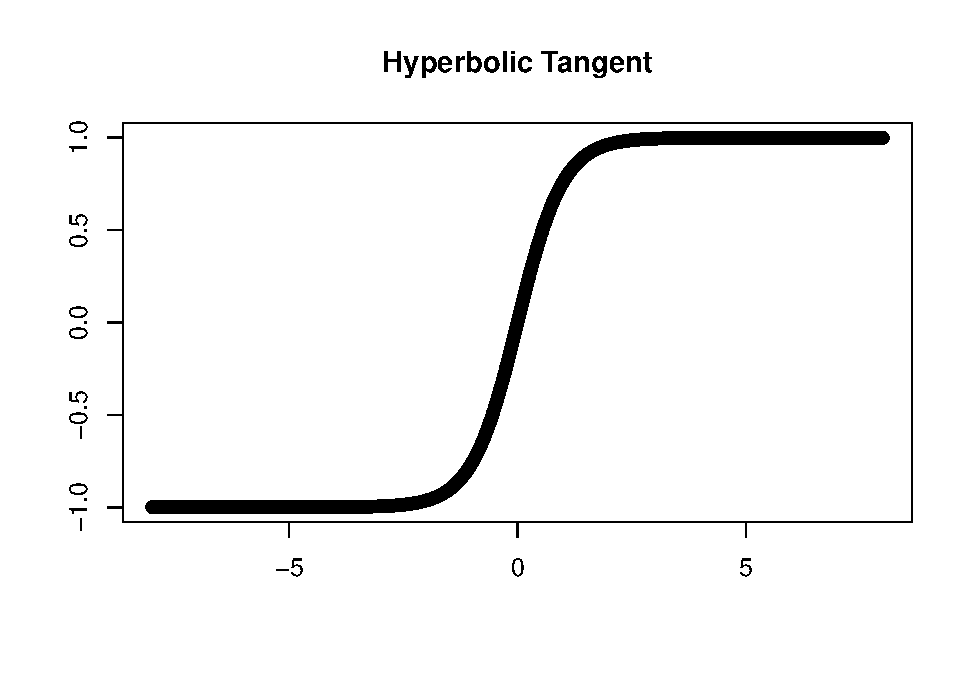
\includegraphics[width=0.5\linewidth]{ANN_files/figures-side-1}
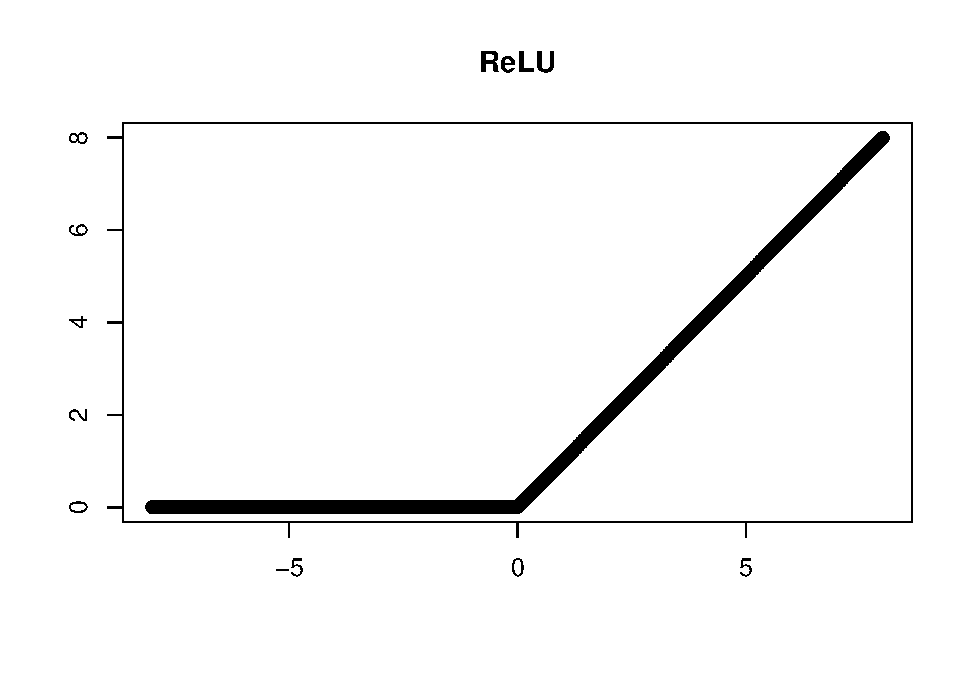
\includegraphics[width=0.5\linewidth]{ANN_files/figures-side-2}

\hypertarget{cost-functions}{%
\subsection{Cost Functions}\label{cost-functions}}

(Change this completely to utilize the correct loss function)

uses the Mean Squared Error loss function to compare true values with
predicted output

\[
C = \frac{1}{n} \sum_{i=1}^N (a^{(L)}_i - y_i)
\] Where \(a^{(L)}_i\) is the outcome of a single iteration of forward
propagation and \(y_i\) is the true observation to compare it to.

\hypertarget{gradient-descent}{%
\subsection{Gradient Descent}\label{gradient-descent}}

The efficiency of a neural network is measured and corrected with each
iteration based on reducing a cost function. This is the same s finding
a local minimum of a function. In a simple case below, given the
function \(f(x) = x^3 + 10x^2\), a loal minimum is found by
differentiating the function.

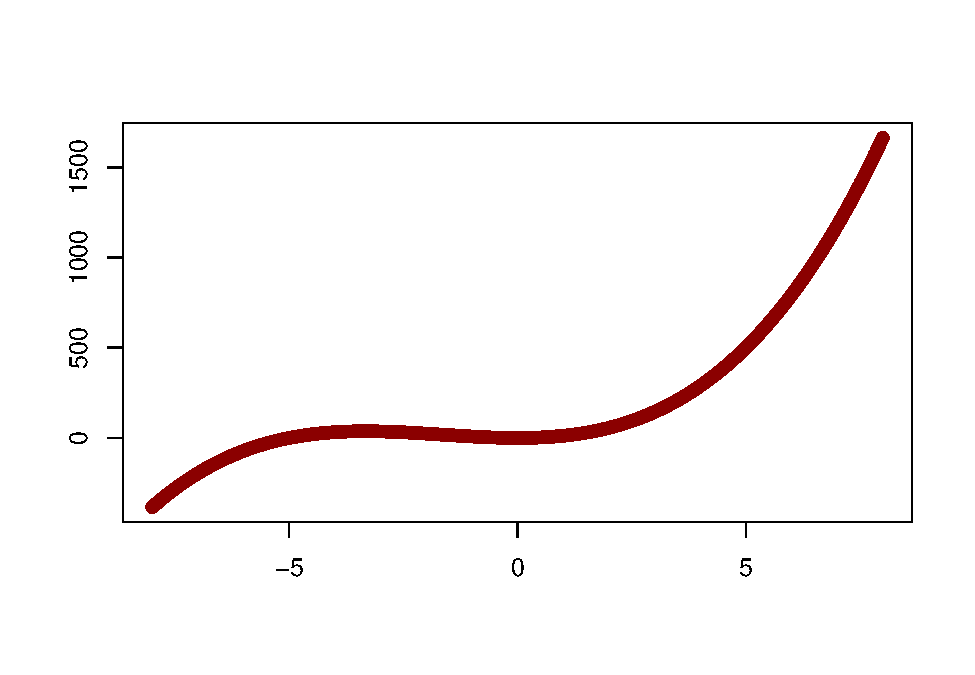
\includegraphics{ANN_files/unnamed-chunk-3-1.pdf}

This is simple when \(x \in \mathbb{R}\), even for
\(x \in \mathbb{R^2}\), but gets more and more complicated as
dimensionality increases to \(x \in \mathbb{R^n}\). This calls for
another means for finding function extrema (particularly minima).
\textbf{Gradient Descent} is the process by which an extrema is found by
means of iterative computation for high-dimensional functions, making it
intrinsically useful for neural networks to learn.

Gradient Descent

\begin{itemize}
\tightlist
\item
  Computes the gradient \$\nabla f(x\_n) =
  \left[ \frac{\partial f}{\partial x_1} , \frac{\partial f}{\partial x_2} , ... , \frac{\partial f}{\partial x_n} \right] \$
\item
  can be thought of as stepping down off a mountain

  \begin{itemize}
  \tightlist
  \item
    each step is that which reduces height the most
  \end{itemize}
\end{itemize}

Also describe Stochastic Gradient Descent to save computation

\hypertarget{backpropagation}{%
\subsection{Backpropagation}\label{backpropagation}}

\textbf{Backpropagation} is the algorithm that computes the gradient for
high-dimensional derivatives for \textbf{gradient descent}, which helps
us reduce the cost function. For a standard neural network, it is
composed of the partial derivatives of the cost function with respect to
each weight in each layer of the network, and each bias in each layer of
the network.

\[
\nabla{C} =
\begin{bmatrix}
\frac{\partial{C}}{\partial{w_1^{(1)}}} & \frac{\partial{C}}{\partial{w_2^{(1)}}} & \cdots & 
\frac{\partial{C}}{\partial{w_i^{(1)}}} \\
\frac{\partial{C}}{\partial{b_1^{(1)}}} & \frac{\partial{C}}{\partial{b_2^{(1)}}} & \cdots & 
\frac{\partial{C}}{\partial{b_i^{(1)}}} \\
\vdots & \vdots & \ddots & \vdots \\
\frac{\partial{C}}{\partial{w_1^{(l)}}} & \frac{\partial{C}}{\partial{w_2^{(l)}}} & \cdots & 
\frac{\partial{C}}{\partial{w_i^{(l)}}} \\
\frac{\partial{C}}{\partial{b_1^{(l)}}} & \frac{\partial{C}}{\partial{b_2^{(l)}}} & \cdots & 
\frac{\partial{C}}{\partial{b_i^{(l)}}} \\
\end{bmatrix}
\] Here, the superscript \(^{(l)}\) denotes the layer of the network and
the subscript \(_i\) denotes a specific parameter within that specific
layer. Since we have two layers, \(^{(2)}\) indicates the hidden layer
and \(^{(1)}\) the input layer.

The backpropagation algorithm is catered to a specific loss function. In
this example, the loss function is defined above as \emph{Mean Squared
Error}. This function takes the difference between the output from the
network and the specified desired output for each observation. To
understand how each parameter that makes up the output must be adjusted,
the algorithm must differentiate every part of it. This is done by use
of the chain rule in calculus. Ultimately, two parameter
differentiations must be computed for each observation in each layer - a
\emph{weight} and a \emph{bias}, as illustrated in the matrix above.

The chain rule is applied when tracing the lineage of influence on the
network's output. In tracing the architecture of the network backwards
(or ``back propagating''), the output is found to be influenced by:

\begin{itemize}
\tightlist
\item
  an activation function in between the hidden layer and the output,
  which is influenced by the resulting computation of the hidden layer
  \emph{weight}, \emph{bias}, and
\item
  an activation function from the previous layer, which is which is
  influenced by the resulting computation of the previous layer
  \emph{weight}, \emph{bias}, and activation of earlier layers.
\end{itemize}

Because our network only has an input and hidden layer, this
``previous'' layer is the input layer, and the ``activation of earlier
layers'' is our input x-value.

\hypertarget{partial-derivatives-with-respect-to-weight}{%
\paragraph{Partial derivatives with respect to
weight}\label{partial-derivatives-with-respect-to-weight}}

The amount we must adjust the weight in the \emph{hidden} layer is
represented by: \$\$ \begin{eqnarray}
\frac{\partial{C}}{\partial{w_i^{(2)}}}    &=&  \dfrac{\partial{z_i^{(2)}}}{\partial{w_i^{(2)}}}
     \dfrac{\partial{a_i^{(2)}}}{\partial{z_i^{(2)}}}
     \dfrac{\partial{C}}{\partial{a_i^{(2)}}} \\
     
 &=& a_i^{(1)} \sigma'(z_i^{(2)}) 2(a_i^{(2)}-y_i) \\
\end{eqnarray} \$\$

Where \(a_n^{(1)}\) is the activation for each observation in the first
(input) layer, \(\sigma'(z_i^{(2)})\) is the derivative of the sigmoid
activation function with respect to each observation in the second
(hidden) layer, \(a_i^{(2)}\) is the activation for each observation in
the hidden layer, and \(y_i\) is the vector of actual training values
this network hopes to achieve.

The amount we must adjust the weight in the \emph{input} layer is
represented by: \$\$ \begin{eqnarray}
\frac{\partial{C}}{\partial{w_i^{(1)}}}    &=& \dfrac{\partial{z_i^{(1)}}}{\partial{w_i^{(1)}}} \dfrac{\partial{a_i^{(1)}}}{\partial{z_i^{(1)}}}  \dfrac{\partial{z_i^{(2)}}}{\partial{a_i^{(1)}}}
     \dfrac{\partial{a_i^{(2)}}}{\partial{z_i^{(2)}}}
     \dfrac{\partial{C}}{\partial{a_i^{(2)}}} \\
     
&=& x_i \sigma'(z_i^{(1)}) w_i^{(2)} \sigma'(z_i^{(2)}) 2(a_i^{(2)}-y_i) \\

\end{eqnarray} \$\$ where \(x_i\) is the input from our training data,
\(\sigma'(z_i^{(1)})\) is the derivative of the sigmoid activation
function with respect to each observation in the input layer,
\(w_i^{(2)}\) is the vector of weights in the hidden layer, and all else
is the same as is in the previous equation.

\hypertarget{partial-derivatives-with-respect-to-bias}{%
\paragraph{Partial derivatives with respect to
bias}\label{partial-derivatives-with-respect-to-bias}}

The amount we must adjust the bias in the \emph{hidden} layer is
represented by: \[
\frac{\partial{C}}{\partial{b_i^{(2)}}}  =  \dfrac{\partial{z_i^{(2)}}}{\partial{b_i^{(2)}}}
     \dfrac{\partial{a_i^{(2)}}}{\partial{z_i^{(2)}}}
     \dfrac{\partial{C}}{\partial{a_i^{(2)}}} \\
\]

Because the bias is a constant, that is
\(\dfrac{\partial{z_i^{(l)}}}{\partial{b_i^{(l)}}} = 1\), our chain-rule
formula simplifies to the following: \[
\frac{\partial{C}}{\partial{b_i^{(2)}}} = 1 \cdot \sigma'(z_i^{(2)}) 2(a_i^{(2)}-y_i) \\
\]

The amount we must adjust the bias in the \emph{input} layer is
represented by: \$\$ \begin{eqnarray}
\frac{\partial{C}}{\partial{b_i^{(1)}}}    &=& \dfrac{\partial{z_i^{(1)}}}{\partial{b_i^{(1)}}} \dfrac{\partial{a_i^{(1)}}}{\partial{z_i^{(1)}}}  \dfrac{\partial{z_i^{(2)}}}{\partial{a_i^{(1)}}}
     \dfrac{\partial{a_i^{(2)}}}{\partial{z_i^{(2)}}}
     \dfrac{\partial{C}}{\partial{a_i^{(2)}}} \\
     
&=& 1 \cdot \sigma'(z_i^{(1)}) w_i^{(2)} \sigma'(z_i^{(2)}) 2(a_i^{(2)}-y_i) \\

\end{eqnarray} \$\$

\end{document}
